\documentclass{article}
\usepackage[utf8]{inputenc}
\usepackage[T1]{fontenc}
\usepackage{graphicx}
\usepackage{hyperref}
\usepackage{geometry}
\geometry{margin=1in}

\title{ESCAPE}
\date{Encyclopaedia Britannica (1771)}

\begin{document}
\maketitle

\section*{Historical source}
\textbf{Entry ID:} \texttt{entry-escape-1473} \\
\textbf{Volume ID:} 149979622 \\
\textbf{Character Count:} 777

\subsection*{Extracted Text}
ESCAPE, in how a violent or privyvation out of
home lawful reflrant, without being delivered by due
course of low. There are two lots of escape, valent
bay and negligent. Voluntary, when a amreth
another for folony, or other crime, and afterwards lets
him go freely by conting, in which cafe, the party
that permits fich escapes and dailyly commended
and multi author for it. Negligent eleceps, on the con-
trany, in where one is arrested, and afterwards deepas
against the will of the perform that arred him, and is
not purified with fresh guards, and treaken before the
person containing lands left fight or him. By fast, it
oy Will. III: C. 26., the keepers of priform conviving at
efecapes final (forter) crois; and in civil cases the flee
rifi's a preferable for the debt.



\section*{Source record}
\begin{itemize}
\item \textbf{Dataset:} \texttt{NationalLibraryOfScotland/encyclopaedia\_britannica\_illustrated}
\item \textbf{Dataset Revision:} \texttt{309f765b1ecc83e0a7f7762e44b4a927a7555443}
\item \textbf{Page ID:} \texttt{britannica:309f765b1ecc83e0a7f7762e44b4a927a7555443:train:1473} \\
  \textbf{Filename:} \texttt{page-1473-b3b602ef6a3d.jpg} \\
  \textbf{Row Index:} 1473 \\
  \textbf{SHA256:} \texttt{b3b602ef6a3d4961...}
\end{itemize}

\begin{figure}[h]
\centering
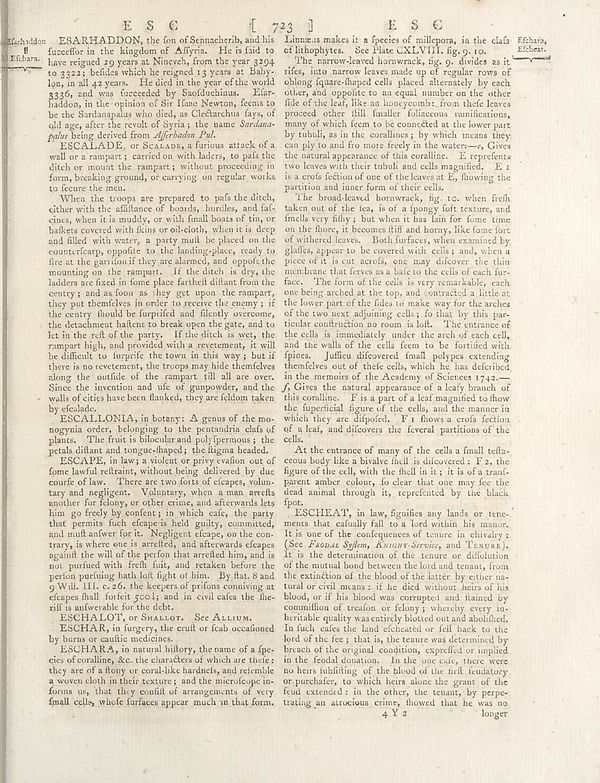
\includegraphics[width=0.85\textwidth]{../scans/page-1473-b3b602ef6a3d.jpg}
\caption*{Source scan: \texttt{page-1473-b3b602ef6a3d.jpg}}
\end{figure}

\end{document}
